\subsection*{Kademlia}

O Kademlia é um \gls*{dht} criado em 2002 \cite{artigo:kademlia} com o objetivo de
melhorar os métodos de busca atuais (Napster e \gls*{gnutella}), que eram ineficientes.
Assim como os outros algoritmos de \gls*{dht}, ele se baseou na estrutura informalmente
conhecida como \enquote{rede de Plaxton} (\emph{Plaxton mesh}), nome que remete a um
dos seus autores \cite{artigo:dht}. Por ter causado boas impressões, foi usado na
implementação da busca de arquivos no programa cliente eMule.

O algoritmo implementa uma rede \emph{overlay} cuja estrutura e comunicação se baseiam
na procura de seus nós. Cada um destes nós é identificado por um identificador único
(ID), que serve tanto para a identificação quanto para a localização de valores na
\gls*{hashtable}.

Outro ponto é que todos os nós são tratados como folhas de uma árvore binária, cujas
posições são estabelecidas pelo menor prefixo comum de seus IDs, e organizando-os de
forma que, para um dado nó $x$, a árvore é dividida em várias subárvores menores que
não o contém. Assim, a maior subárvore consiste de metade da árvore que não contém $x$,
a subárvore seguinte é feita da metade da árvore restante onde $x$ também não está
contido, etc. O Kademlia garante ainda que todo nó conhece um outro que está em cada
uma das subárvores, se estas contiverem algum nó.

\begin{figure}[ht!]
    \centering
    \fbox{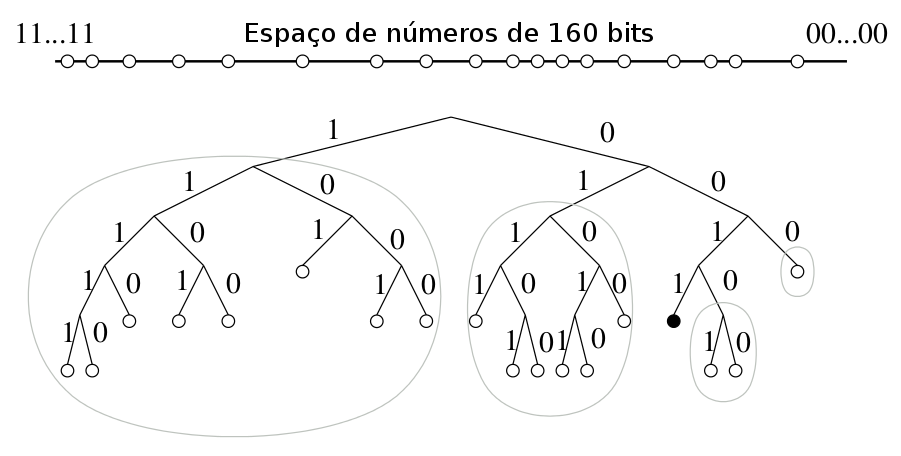
\includegraphics[width=\textwidth]{dht1.png}}
    \caption{Árvore binária do Kademlia. O nó preto é a posição do ID 0011...; os ovais
    cinzas são as subárvores onde o nó preto deve possuir nós conhecidos. Fonte:
    \cite{artigo:kademlia}}
    \label{fig:dht-arvore}
\end{figure}

Durante uma busca, o processo deve conhecer a chave (que é um
\gls*{hashvalue}) associado ao objeto - neste caso, o ID do \gls*{torrent}, que é seu
\gls*{hashvalue} - e explora a rede em passos, encontrando nós mais próximos da chave,
até encontrar o valor buscado ou não nós existirem mais próximos que o atual. Dessa
forma, para uma rede com $n$ nós, o algoritmo visita apenas $O(\log n)$ nós.

\begin{figure}[ht!]
    \centering
    \fbox{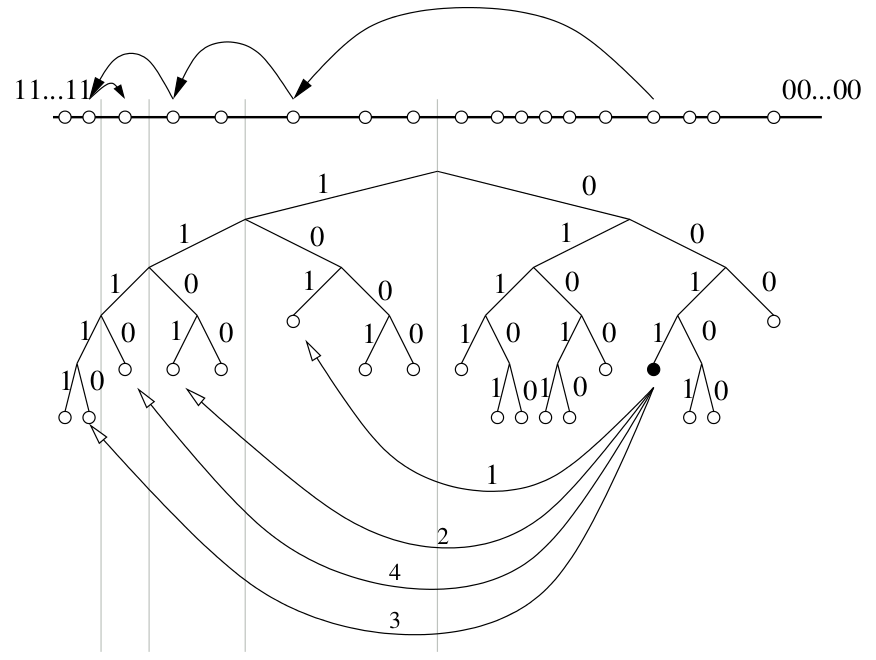
\includegraphics[width=\textwidth]{dht2.png}}
    \caption{Exemplo de uma busca na árvore de nós do Kademlia usando-se um ID. O nó
    preto, de prefixo 0011, encontra o nó de prefixo 1110 através de sucessivas buscas
    (setas numeradas inferiores). As setas superiores mostram a convergência da
    busca durante a execução. Fonte: \cite{artigo:kademlia}}
    \label{fig:dht-arvore-busca}
\end{figure}

\subsection*{Funcionamento}

No Kademlia, objetos e nós possuem IDs únicos de 160 bits: enquanto o primeiro utiliza
o \gls*{hashvalue} de 20 bytes SHA-1 da chave \bverb|info_hash| do \gls*{torrentfile},
o segundo é um valor aleatório escolhido pelo próprio programa.

As distâncias entre nós são calculadas usando-se a função de distância

\begin{equation}
    d(x,y) = x \oplus y
\end{equation}

que possui algumas propriedades em comum com a equação de distância euclidiana usual,
como as seguintes:

\begin{itemize}
    \item $d(x,x) = 0$
    \item $x \neq y$, $d(x,y) > 0$
    \item simetria: $\forall x,y$, $d(x,y) = d(y,x)$
    \item desigualdade triangular: $d(x,y) + d(y,z) \geq d(x,z)$. \\
        Isto vem do fato de $d(x,z) = d(x,y) \oplus d(y,z)$ e que $\forall a \geq 0,
        \forall b \geq 0 : a + b \geq a \oplus b$
    \item unidirecionalidade: para um dado ponto $x$ e uma distância $\Delta > 0$,
        existe exatamente um ponto $y$ tal que $d(x,y) = \Delta$. Isso garante que todas
        as procuras por uma mesma chave convirjam para um mesmo percurso, independente
        do ponto de partida.
\end{itemize}

\subsubsection*{Estado dos nós}

Cada nó do Kademlia armazena informações sobre outros nós para rotear mensagens de
pesquisa. Para cada bit $i$ dos IDs (cada ID tem 160 bits) é mantido um \gls{kbucket},
que contém os nós cuja distância até ele está entre $2^i$ e $2^{i+1}$. Esses
\glspl*{kbucket} são listas de endereço IP, porta de comunicação \gls*{udp} e ID de
nós, ordenadas pelo horário da última notícia destes. Para distâncias pequenas, essas
listas geralmente serão vazias, enquanto para distâncias maiores poderão ser de tamanho
$k$. Este valor, que é o de replicação do sistema, é escolhido de tal forma que esses
$k$ nós possuam grande probabilidade de não falharem na próxima hora.

Quando um nó \textbf{A} recebe uma mensagem de outro nó \textbf{B}, o \gls*{bucket}
correspondente ao ID do remetente (nó \textbf{B}) é atualizado. Disto, podem ocorrer as
seguintes situações:

\begin{itemize}
    \item \textbf{B} já existe no \gls*{bucket}: passa a ser o primeiro da lista, pois
        existiu mensagem recente.

    \item \textbf{B} não existe no \gls*{bucket}:
        \begin{itemize}
            \item \gls*{bucket} não está cheio: \textbf{B} é adicionado no começo da
                lista.
            \item \gls*{bucket} cheio: é enviado um \emph{ping} para o nó do final da
                lista (nó \textbf{C}), contatado há mais tempo

            \begin{itemize}
                \item \textbf{C} não responde ao \emph{ping}: \textbf{C} é retirado da
                lista e \textbf{B} é inserido no início
                \item \textbf{C} responde ao \emph{ping}: \textbf{C} é movido para o
                início da lista e \textbf{B} é ignorado
            \end{itemize}
        \end{itemize}

\end{itemize}

Por conta disso, ocorre que nós mais antigos e funcionais são preferidos, pois quanto
mais tempo um nó está conectado, mais provável ele se manterá conectado por mais 1 hora
\cite{artigo:gnutella-uptime}. Outra vantagem disso é a resistência a alguns ataques de
negação de serviço, pois mesmo que ocorra uma inundação de novos nós, estes só seriam
inseridos nos \glspl*{kbucket} se os antigos fossem excluídos.

\subsubsection*{Protocolo}

O protocolo de mensagens \gls*{dht} utiliza o formato KRPC, que é um mecanismo de
chamada \gls{rpc} que envia dicionários \gls*{bencode} através de \gls*{udp}, uma única
vez por chamada (um pacote para a requisição, outro para a resposta), sem novas
tentativas.

Existem 3 tipos de mensagem: consulta (\emph{query}), resposta (\emph{response}) e erro
(\emph{error}). Para o protocolo \gls*{dht}, são 4 comandos \emph{query}: \bverb|ping|,
\bverb|find_node|, \bverb|get_peers| e \bverb|announce_peer|. Em todos, o nó sempre
enviará seu ID como valor da chave \bverb|id|.

Uma mensagem KRPC é um dicionário com 2 chaves comuns a todos os 4 comandos: \bverb|y|,
que especifica o tipo da mensagem, e \bverb|t|, que corresponde ao ID da transação.
Este é um número binário convertido para \gls*{string}, geralmente formada por 2
caracteres, possuindo valor até $2^{16}$, e devolvida nas respostas. Isso permite que
estas se relacionem a múltiplas consultas a um nó. Esse ID é chamado de \emph{magic
\gls{cookie}} (cookie mágico) \cite{wiki:magic-cookie}.

Cada tipo de mensagem possui formatos diferentes entre si, permitindo parâmetros
adicionais para cada chamada, possuindo as seguintes chaves e seus respectivos valores:

\newpage
\begin{itemize}
    \item \emph{query}
        \begin{itemize}
            \item \bverb|y|: caractere \sverb|q|
            \item \bverb|q|: string do comando desejado (\sverb|ping|,
                \sverb|find_node|, \sverb|get_peers|, \sverb|announce_peer|)
            \item \bverb|a|: dicionário contendo parâmetros adicionais, dependendo do
                comando passado na chave \bverb|q|
        \end{itemize}

    \item \emph{response}
        \begin{itemize}
            \item \bverb|y|: caractere \sverb|r|
            \item \bverb|r|: dicionário contendo valores da resposta, dependendo do
                comando passado na chave \bverb|q|
        \end{itemize}

    \item \emph{error}
        \begin{itemize}
            \item \bverb|y|: caractere \sverb|e|

            \item \bverb|e|: lista contendo 2 elementos: código (número inteiro) e
                mensagem para o erro (\gls*{string}). Os erros podem ser:
                \begin{itemize}
                    \item 201 (Generic Error): erros genéricos
                    \item 202 (Server Error): erros de servidor
                    \item 203 (Protocol Error): para pacote mal formado, argumento
                        inválido ou token incorreto
                    \item 204 (Method Unknown): comando não conhecido
                \end{itemize}

            \item exemplo: \\
                \bverb|d1:eli201e23:A Generic Error Ocurrede1:t2:aa1:y1:ee|
                (\gls*{bencode}) \\
                \sverb|{"t":"aa", "y":"e", "e":[201, "A Generic Error Ocurred"]}|
                (\gls*{string})
        \end{itemize}
\end{itemize}

As informações retornadas podem ser sobre \glspl*{peers} ou nós \gls*{dht}: enquanto o
primeiro é a \enquote{informação compacta de endereço IP/porta} - string de 6 bytes (4
bytes iniciais para o endereço IP e 2 bytes finais para a porta de comunicação usada)
-, o segundo é a \enquote{informação compacta de nó} - string de 26 bytes (20 bytes
iniciais para o ID do nó e 6 bytes finais para a respectiva informação compacta de
endereço IP/porta).

\subsubsection*{Comandos}

Os 4 comandos de \emph{query} do \gls*{dht} (\bverb|ping|, \bverb|find_node|,
\bverb|get_peers| e \bverb|announce_peer|) estão definidos da seguinte forma.

% \newpage
\subsubsubsection{ping}

É o comando mais simples, que verifica se o nó está online. Possui um único argumento,
que é uma chave \bverb|id|, que é o ID do nó consultante (na requisição) ou do nó
consultado (na resposta).

\begin{itemize}
    \item formato da requisição \\
        \bverb|d1:ad2:id20:abcdefghij0123456789e1:q4:ping1:t2:aa1:y1:qe|
        (\gls*{bencode}) \\
        \sverb|{"t":"aa", "y":"q", "q":"ping", "a":{"id":"abcdefghij0123456789"}}|
        (\gls*{string})

    \item formato da resposta \\
        \bverb|d1:rd2:id20:mnopqrstuvwxyz123456e1:t2:aa1:y1:re|
        (\gls*{bencode}) \\
        \sverb|{"t":"aa", "y":"r", "r":{"id":"mnopqrstuvwxyz123456"}}|
        (\gls*{string})
\end{itemize}

\cfile[label="./third-party/dht/dht.c:2291"]{./Codes/chap3/016-dht-macros.c}
\cfile[label="./third-party/dht/dht.c:2341"]{./Codes/chap3/017-dht-ping.c}

\newpage
\subsubsubsection{find\_node}

Este comando, que equivale à mensagem de \bverb|FIND\_NODE| do artigo do Kademlia
\cite{artigo:kademlia}, é usado para encontrar as informações do nó dado seu ID.
Necessita enviar 2 argumentos: a chave \bverb|id| e o ID do nó consultante, e a chave
\bverb|target| e o ID do nó cujas informações o consultante está procurando (ou nó
alvo).

\begin{itemize}
    \item formato dos argumentos da requisição \\
        \sverb|{"id":\"<IDs dos nós consultantes>", "target":\"<ID do nó alvo>"}|

    \item formato da resposta \\
        \sverb|{"id":\"<IDs dos nós consultados>", "nodes":\"<info compacta do(s) nó(s)>"}|
\end{itemize}

O nó consultado deve responder com a chave \bverb|nodes| contendo uma
\gls*{string} com a informação compacta (6 bytes) do nó alvo ou dos $k$ nós bons (que
fizeram contato recentemente) mais próximos que estão contidos em sua tabela de
roteamento, de 1 ou mais \glspl*{kbucket}. O funcionamento do algoritmo da busca é
explicado no trabalho:

\blockquote{O procedimento mais importante que um participante do Kademlia deve realizar
é encontrar os $k$ nós próximos a um dado ID de nó. Nós chamamos esse procedimento de
\enquote{\emph{lookup} de nós}. Kademlia utiliza de um algoritmo recursivo nas buscas
por nós. O disparador das buscas começa escolhendo $\alpha$ nós do \gls*{bucket} não-
vazio mais próximo (ou, se esse \gls*{bucket} tiver menos que $\alpha$ entradas,
utiliza desses $\alpha$ nós mais próximos que conhece). Então, o disparador envia
chamadas \gls*{rpc} assíncronas paralelas de comandos \textbf{find\_node} para esses
$\alpha$ nós escolhidos. $\alpha$ é um parâmetro de concorrência geral ao sistema,
assumindo valor como 3.

No passo recursivo, o disparador reenvia chamadas a \textbf{find\_node} para os nós que
conheceu das chamadas \gls*{rpc} passadas. (Esta recursão pode começar antes que todos
os $\alpha$ nós anteriores tenham respondido). Dos $k$ nós que o disparador concluiu
serem mais próximos ao alvo, ele pega $\alpha$ que ainda não foram consultados e envia
chamadas \gls*{rpc} \textbf{find\_node}. Nós que falharem em responder rapidamente são
desconsiderados até que respondam. Se uma rodada de comandos \textbf{find\_node} não
retornar algum nó mais próximo do que os nós já conhecidos, o disparador reenvia
comandos \textbf{find\_node} para todos os $k$ nós mais próximos que ainda não foram
consultados. O \emph{lookup} termina quando o disparador tiver consultado e obtido
respostas de todos os $k$ nós mais próximos conhecidos.}

Porém, o Transmission implementa essa busca de forma mais flexível e simples. De início,
busca o \gls*{bucket} no qual o ID procurado está ou que contém nós mais próximos.

\cfile[label="./third-party/dht/dht.c:2536"]{./Codes/chap3/020-dht-sendclosestnodes.c}

A busca do \gls*{bucket} itera sobre a lista ligada de \glspl*{bucket}.

\cfile[label="./third-party/dht/dht.c:129"]{./Codes/chap3/018-dht-structs.c}
\cfile[label="./third-party/dht/dht.c:464"]{./Codes/chap3/019-dht-findbucket.c}

Caso retorne o \gls*{bucket} mais provável, efetua buscas internas nele. Se ele possuir
elementos vizinhos anteriores ou posteriores, também busca por nós neles.

\cfile[label="./third-party/dht/dht.c:2523"]{./Codes/chap3/021-dht-bufferclosestnodes.c}
\cfile[label="./third-party/dht/dht.c:2476"]{./Codes/chap3/022-dht-insertclosestnode.c}

Ao fim da busca, envia a lista de nós que encontrou como resposta ao comando de
\bverb|find_node| recebida. O Transmission também utiliza a função para enviar os nós
encontrados pelo comando \bverb|get_peers| (pág. ~\pageref{subsubsubsec:getpeers}).

\cfile[label="./third-party/dht/dht.c:2409"]{./Codes/chap3/023-dht-sendnodespeers.c}

Um exemplo de requisição e resposta para este comando é

\begin{itemize}
    \item exemplo de requisição \\
        \bverb|d1:ad2:id20:abcdefghij01234567896:target20:mnopqrstuvwxyz123456e1:q| \\
        \bverb|9:find_node1:t2:aa1:y1:qe| (\gls*{bencode}) \\
        \sverb|{"t":"aa", "y":"q", "q":"find_node", "a":{"id":"abcdefghij0123456789",| \\
        \sverb|"target":"mnopqrstuvwxyz123456"}}| (\gls*{string})

    \item exemplo de resposta \\
        \bverb|d1:rd2:id20:0123456789abcdefghij5:nodes9:def456...e1:t2:aa1:y1:re| \\
        (\gls*{bencode}) \\
        \sverb|{"t":"aa", "y":"r", "r":{"id":"0123456789abcdefghij", "nodes":| \\
        \sverb|"def456..."}}| (\gls*{string})
\end{itemize}

\subsubsubsection{get\_peers}
\label{subsubsubsec:getpeers}

É o comando \gls*{rpc} da mensagem \bverb|FIND_VALUE|, serve para buscar \glspl*{peer}
para um dado um \gls*{hashvalue} identificador de \gls*{torrentfile}, enviado como
valor da chave \bverb|info_hash|, além do ID do nó consultante como valor da chave
\bverb|id|.

O funcionamento é equivalente ao comando \bverb|find_node|, com um detalhe extra: se o
nó que recebeu a mensagem possuir \glspl*{peer} para o \gls*{hashvalue} dado, eles são
informados imediatamente na forma compacta (6 bytes para cada \gls*{peer}) numa lista
\gls*{bencode} de \glspl*{string}, devolvida como valor da chave \bverb|values|. Por
outro lado, caso o receptor da mensagem não conhecer nós para o \gls*{hashvalue}
especificado, a resposta conterá a chave \bverb|nodes| com os $k$ nós mais próximos
desse \gls*{hashvalue}. O nó original consulta outros nós próximos ao \gls*{torrentfile}
iterativamente. Ao fim da busca, o programa cliente insere o contato para si mesmo na
lista de nós próximos ao \gls*{torrentfile}.

Em ambos os casos, uma chave \bverb|token| é informada na resposta, cujo valor é uma
\gls*{string} binária curta, que deverá ser utilizada em futuras mensagens de
\bverb|announce_peer|.

\todoquestion{referencio o código do comando anterior?}

\begin{itemize}
    \item formato dos argumentos da requisição \\
        \sverb|{"id":\"<IDs dos nós consultantes>",| \\
        \sverb| "info_hash":\"<hash de 20 bytes do torrent buscado>"}|

    \item formato da resposta \\
        \sverb|{"id":\"<IDs dos nós consultados>", "token":\"<token>",| \\
        \sverb| "values":[\"<info peer 1>", \"<info peer 2>", ...]}| \\
        ou \\
        \sverb|{"id":\"<IDs dos nós consultados>", "token":\"<token>",| \\
        \sverb| "nodes":\"<info compacta do(s) nó(s)>"}| \\ \\
\end{itemize}

\cfile[label="./third-party/dht/dht.c:1866"]{./Codes/chap3/024-dht-periodic.c}

\newpage
\begin{itemize}
    \item exemplo de requisição \\
        \bverb|d1:ad2:id20:abcdefghij01234567899:info_hash20:mnopqrstuvwxyz123456e|\\
        \bverb|1:q9:get_peers1:t2:aa1:y1:qe| (\gls*{bencode}) \\
        \sverb|{"t":"aa", "y":"q", "q":"get_peers",|\\
        \sverb| "a":{"id":"abcdefghij0123456789", "info_hash":"mnopqrstuvwxyz123456"}}| (\gls*{string})

    \item exemplo de resposta
        \begin{itemize}
            \item com peers \\
                \bverb|d1:rd2:id20:abcdefghij01234567895:token8:aoeusnth|\\
                \bverb|6:valuesl6:axje.u6:idhtnmee1:t2:aa1:y1:re| (\gls*{bencode}) \\
                \sverb|{"t":"aa", "y":"r", "r":{"id":"abcdefghij0123456789",|\\
                \sverb| "token":"aoeusnth", "values":["axje.u", "idhtnm"]}}|
                (\gls*{string})

            \item com nós próximos \\
                \bverb|d1:rd2:id20:abcdefghij01234567895:nodes9:def456...5:token|\\\bverb|8:aoeusnthe1:t2:aa1:y1:re| (\gls*{bencode}) \\
                \sverb|{"t":"aa", "y":"r", "r":{"id":"abcdefghij0123456789",|\\
                \sverb| "token":"aoeusnth", "nodes":"def456..."}}| (\gls*{string})
        \end{itemize}
\end{itemize}

\subsubsubsection{announce\_peer}

O último comando é o da mensagem \bverb|STORE|, pelo qual um nó avisa outros que está
baixando um \gls*{torrentfile}, passando 4 argumentos: o ID do nó consultante como
valor da chave \bverb|id|, o \gls*{hashvalue} identificador do \gls*{torrentfile} na
chave \bverb|info_hash|, \bverb|port| contém um número inteiro de porta, e o
\bverb|token| recebido como resposta de uma mensagem \bverb|get_peers| anterior. O nó
consultado deve verificar que esse token foi enviado anteriormente para o mesmo endereço
IP que o nó consultante, e então o nó consultado armazena usando o \bverb|info_hash| do
torrent como chave e a informação compacta de endereço IP/porta do nó como valor.

Existe ainda mais um argumento, opcional, que é o \bverb|implied_port|, cujo valor pode
ser 0 ou 1. Se este for 1, o argumento da porta deve ser ignorado e então a fonte de
pacotes \gls*{udp} deve ser usada como a porta do \gls*{peer}. Isso é útil para
\glspl*{peer} que estão em redes internas a \gls{nat}, que podem não saber quais são
suas portas externas, e que suportam uTP, aceitando conexões na mesma porta que o
\gls*{dht}.

O token tem papel fundamental para a segurança neste comando, pois serve para prevenir
que um \gls*{peer} malicioso registre outros \glspl*{peer} para um \gls*{torrenfile}.
No BitTorrent, esse token é a \gls*{string} do \gls*{hashvalue} SHA-1 do endereço IP
concatenado a uma chave secreta, criada pelo programa cliente, que varia a cada 5
minutos e são aceitos até 10 minutos depois de serem criados.

\newpage
\begin{itemize}
    \item formato dos argumentos da requisição \\
        \sverb|{\"id": \"<IDs dos nós consultantes>",| \\
        \sverb| \"implied_port": <0 ou 1>,| \\
        \sverb| \"info_hash": \"<hash de 20 bytes do torrent>",| \\
        \sverb| \"port": <número da porta>,| \\
        \sverb| \"token": \"<token>"}|

    \item formato da resposta \\
        \sverb|{"id": \"<IDs dos nós consultados>"}|
\end{itemize}

\cfile[label="./third-party/dht/dht.c:1277"]{./Codes/chap3/025-storage-store.c}

\begin{itemize}
    \item exemplo de requisição \\
        \bverb|d1:ad2:id20:abcdefghij01234567899:info_hash20:mnopqrstuvwxyz123456| \\
        \bverb|4:porti6881e5:token8:aoeusnthe1:q13:announce_peer1:t2:aa1:y1:qe| \\
        (\gls*{bencode}) \\
        \sverb|{"t":"aa", \"y":"q", \"q":"announce_peer",| \\
        \sverb|"a":{"id":"abcdefghij0123456789", \"implied_port": 1,| \\
        \sverb|"info_hash":"mnopqrstuvwxyz123456", \"port": 6881, \"token": \"aoeusnth"}}|
        (\gls*{string})

    \item exemplo de resposta \\
        \bverb|d1:rd2:id20:mnopqrstuvwxyz123456e1:t2:aa1:y1:re| \\
        (\gls*{bencode}) \\
        \sverb|{"t":"aa", \"y":"r", \"r": {"id":"mnopqrstuvwxyz123456"}}|
        (\gls*{string})
\end{itemize}

% ===========================================================================